\setchapterpreamble[u]{\margintoc}
\chapter{High Energy {\sffamily QCD}}
\labch{qcd}

\begin{preview}[]
Some basic concepts of {\sffamily} QCD shall briefly be presented, with focus on gauge transformations and Yang-Mills equations. The formulation and quantization of chromodynamics using light-cone coordinates will schematically be provided, with detailed proofs in \refapp{appendixlc}. Afterwards, an overview of high-energy {\sffamily QCD} and the small-$x$ physics which arise from {\sffamily DIS} will be given. 
\end{preview}

\section{{\sffamily QCD}}
Quantum chromodynamics is the theory of strong interactions.\sidenote{A brief historical review about the development of {\sffamily QCD} may be found at \cite{historyqcd}.}It aims to describe the interactions between elementary constituents, namely the quarks,\sidenote{The quarks were firstly predicted in Gell-Mann's Eightfold Way \cite{gellmann}.}mediated by the carriers of the color force, the gluons. \\ 
The existence of color charge was proposed as an additional quantum number which would solve the violation of Pauli's exclusion principle for some particular baryons.\sidenote{For example, $\Delta^{++}$, which consists of three up quarks.}Since the quarks were never experimentally evidenced, it was proposed that the strong interaction constrains the free particles to only exist in color neutral states. This particularity of {\sffamily QCD} is known as color confinement. Nevertheless, in the partonic picture,\sidenote{Feynman proposed that high energy nuclei are made of elementary constituents, generically called partons \cite{partons}.}deep inelastic scattering\sidenote{{\sffamily DIS} is a process during which the structure of a hadron may be probed via interaction with, in general, a lepton.}experiments between an electron and a proton confirmed the already predicted Bjorken scaling\sidenote{Bjorken deduced an expression for the cross-section of the electron by imagining that it interacts electromagnetically with each parton from the proton \cite{bjorkenimf}.}of the electrons' differential cross-section. \\
In essence, {\sffamily QCD} is an extension of the original $\textsf{SU}(2)$ gauge theory of Yang and Mills \cite{yangmills} to local non-Abelian $\textsf{SU}(3)$ gauge transformations.

\subsubsection*{Field content}
Following textbook expositions \cite{maggiore, peskin, greiner}, the {\sffamily QCD} Lagrangian $\mathcal{L}$ is constructed from symmetry principles, namely $\textsf{SO}(1,3)$ Lorentz invariance and local gauge invariance under $\textsf{SU}(3)$. The fields should transform according to irreducible representations of these groups. The quark content of the Lagrangian is described by the quark and anti-quark fields $\psi_{\alpha,i,f}(x)$ and $\overline{\psi}_{\alpha,i,f}(x)$. They are Dirac spinors (spinorial index $\alpha$), transform according to the fundamental representation of $\textsf{SU}(3)$ (color index $i=1,2,3$ or red, green, blue) and come in different flavours (flavour index $f=\overline{1,N_f}$ or up, down, strange, charm, bottom, up). The gluon fields $A_a^\mu(x)$ are Lorentz vectors and each correspond to a generator $t^a$ ($a=\overline{1,8}$) which, in the fundamental representation, is given by the Gell-Mann matrices $t^a=\lambda^a/2$.

\subsubsection*{Gauge transformations} 
The quark and anti-quark fields must be invariant under local $\textsf{SU}(3)$ gauge transformations\sidenote{For simplicity, all the field indices will be dropped in the following computations.}
\coloredeq{
    \psi(x)\mapsto\textsf{U}(x)\psi(x), \quad \overline{\psi}\mapsto\overline{\psi}(x)\textsf{U}^\dagger(x), 
}
with the group transformation expressible, via exponentiation, from the Lie algebra generators, with space-time dependent group parameters $\varepsilon^a(x)$, as 
\begin{equation}\label{qcd13}
    \textsf{U}(x)=\exp{i\sum_a\varepsilon^a(x)t^a}.
\end{equation}
The gauge fields\sidenote{For each algebra element $t^a$, one may introduce a gauge field $A_a^\mu$. These may be then used to construct a Lie-algebra valued gauge potential $A^\mu$. This potential depends on the chosen representation.}$A_\mu(x)=\sum\limits_a A^a_\mu(x)t^a$ must transform according to
\coloredeqnum{qcd11}{
    A_\mu(x)\mapsto\textsf{U}(x)A_\mu(x)\textsf{U}^\dagger(x)+\frac{i}{g}\textsf{U}(x)\big[\partial_\mu\textsf{U}^\dagger(x)\big],
}
where $g$ denotes the coupling constant. It is important to notice that one may generate gluon fields out of a null one, that is $A_\mu=0$ by applying a local gauge transformation. Such field configurations take the form
\begin{equation}\label{qcd10}
    A_\mu^{\text{pure}}=\frac{i}{g}\textsf{U}\big(\partial_\mu\textsf{U}^\dagger\big)
\end{equation}
and are called pure gauge fields \cite{gelisqft,eichmann}. The corresponding field strength tensor is null $F_{\mu\nu}^{\text{pure}}=0$. \\
Let us now introduce the covariant derivative\sidenote{The covariant derivative has an elegant geometrical interpretation \cite{torre}: it represents the rate of change when fields from different space-time points are parallel transported along a given path. During this procedure, they are being aligned such that they may be properly compared. The corresponding connection is actually the gauge field.}
\begin{equation*}
    \textsf{D}_\mu=\partial_\mu-igA_\mu. 
\end{equation*}
Further, one may define the field strength tensor as the commutator between covariant derivatives\sidenote{Since it arises as a commutator between covariant derivatives, which describe the parallel transport, the field strength tensor may be interpreted as a measure of the path dependence of parallel transport. For this reason, it is also referred to as the curvature \cite{torre}.}
\begin{equation*}
    F_{\mu\nu}=\frac{i}{g}\big[\textsf{D}_\mu,\textsf{D}_\nu\big],
\end{equation*}
which yields an expression in terms of gauge fields
\coloredeqnum{qcd2}{
    F_{\mu\nu}=\partial_\mu A_\nu-\partial_\nu A_\mu-ig\big[A_\mu,A_\nu\big],
}
or equivalently, by color components $F_{\mu\nu}=F_{\mu\nu}^at^a$, as
\begin{equation*}
    F_{\mu\nu}^a=\partial_\mu A_\nu^a-\partial_\nu A_\nu^a+gf^{abc}A_\mu^bA_\nu^c,
\end{equation*}
where $f^{abc}$ are the structure constants of the Lie algebra $\mathfrak{su}(3)$. The last term from the above equation, when plugged in the Lagrangian, will give rise to gluonic self-interactions, a particular feature of QCD. The field strength tensor gauge transforms in the usual manner as
\coloredeq{
    F_{\mu\nu}(x)\mapsto \textsf{U}(x)F_{\mu\nu}(x)\textsf{U}^\dagger(x).
}

\subsubsection*{{\sffamily QCD} Lagrangian} 
We may now proceed to constructing the Lagrangian. The quark content is that of a free fermionic Lagrangian,\sidenote{After replacing the partial derivative with the covariant derivative, the Lagrangian will also contain an interaction term
\begin{equation*}
    \mathcal{L}_{\textsf{int}}=g \overline{\psi} \gamma^\mu A_\mu^a t^a \psi.
\end{equation*}}but built with covariant derivatives, in order to satisfy gauge invariance
\begin{equation}\label{qcd1}
    \mathcal{L}_{\textsf{quarks}}=\overline{\psi}(x)\big(i\slashed{\textsf{D}}-\textsf{M}\big)\psi(x),
\end{equation}
where $\textsf{M}=\textsf{Diag}\left\{m_1,\ldots,m_{N_f}\right\}$ is the diagonal quark mass matrix in flavour space.\sidenote{In the Standard Model, the quark mass matrix is no longer diagonal. After spontaneous symmetry breaking, the mixing between different flavoured quark masses is given by the CKM matrix \cite{pdg}.} \\
The dynamics of the gluon fields is described by the following construction\sidenote{It is important to notice that such a construction contains not only standard kinetic terms but also interaction vertices with three gluons, which are proportional to $g$ and four gluons, proportional to $g^2$.}
\begin{equation}\label{qcd12}
    \mathcal{L}_{\textsf{gluons}}=-\frac{1}{2}\textsf{Tr}\left\{F_{\mu\nu}F^{\mu\nu}\right\},
\end{equation}
where the color tracing over the contraction of field strength tensors assured gauge invariance. Equivalently, one may rewrite the above expression in terms of color components as
\begin{equation}\label{qcd3}
    \mathcal{L}_{\textsf{gluons}}=-\frac{1}{4}F_{\mu\nu}^aF^{a,\mu\nu},
\end{equation}
valid in the fundamental representation, where $\textsf{Tr}\left\{t^at^b\right\}=\delta^{ab}/2$. Therefore, the {\sffamily QCD} Lagrangian takes the form
\coloredeqnum{qcd6}{
    \mathcal{L}_{\textsf{QCD}}=\overline{\psi}(x)\big(i\slashed{\textsf{D}}-\textsf{M}\big)\psi(x)-\frac{1}{4}F_{\mu\nu}^aF^{a,\mu\nu}.
}

\subsubsection*{Field equations} 
The variational derivatives with respect to the color spinor fields give the colored Dirac equations
\begin{equation}\label{qcd4}
    (i\slashed{\textsf{D}}-\textsf{M})\psi=0,    
\end{equation}
and similarly for the anti-quark fields
\begin{equation*}
    \overline{\psi}(i\overleftarrow{\slashed{\textsf{D}}}-\textsf{M})=0.    
\end{equation*}
The Euler-Lagrange equations corresponding to the gluon fields yield the Yang-Mills equations, or equivalently, colored Maxwell equations\sidenote{There is an additional equation, called the Bianchi identity, which follows from the definition and properties of $F_{\mu\nu}$. It may be expressed as \cite{tong}
\begin{equation}\label{qcd5}
    \textsf{D}_\mu^{\phantom{*}*}F^{\mu\nu}=0,
\end{equation}
where we introduced the dual field strength tensor as
\begin{equation*}
    ^*F^{\mu\nu}=\frac{1}{2}\epsilon^{\mu\nu\rho\sigma}F_{\rho\sigma}.
\end{equation*}}
\coloredeqnum{qcd9}{
    \textsf{D}_\nu F^{\nu\mu}=gJ^\mu,
}
in which $J^\mu=\sum\limits_a J^{a,\mu} t^a$ with $J^{a,\mu}=\overline{\psi}\gamma^\nu t^a\psi$ being the color current. The color current is covariantly conserved $\textsf{D}_\mu J^\mu=0$.

\section{Light-cone {\sffamily QCD}}
Further, the light-cone quantization of chromodynamics\sidenote{As opposed to the standard quantization, done in the framework of path integrals \cite{schwartz}. We shall see that this approach brings considerable simplifications and there will be no need for Faddeev-Popov ghosts \cite{brodsky}.} shall briefly be presented.\sidenote{Detailed computations may be found in \refapp{appendixlc}.}For this purpose, we are going to work in one of the forms of relativistic dynamics proposed by Dirac \cite{reldyn}, namely the {\sffamily\color{ming} light-front form}, by using {\sffamily\color{ming} light-cone coordinates} defined as\sidenote{We are going to use the Kogut-Soper convention \cite{brodsky}. There also exists the Lepage-Brodsky choice for defining these coordinates as $x^\pm\overset{\Delta}{=}x^0\pm x^3$. Even though quantities such as the Dirac matrices, projection operators, Dirac spinors, polarization vectors and others differ in these conventions, the final results remain the same.}
\coloredeqnum{qcd8}{
    x^\pm\overset{\Delta}{=}\frac{1}{\sqrt{2}}\left(x^0\pm x^3\right).
}

\begin{marginfigure}[-5.5cm]
	\centering
    \includesvg[width=\textwidth]{images/diagrams/lc_coord.svg}
    \caption*{Diagram of light-cone and cartesian coordinates.}
\end{marginfigure}

The Poincar\'e group in light-cone coordinates possesses a sub-group isomorphic to the two-dimensional Galilean group. For this reason, one may attribute the following physical interpretations \cite{venugopalanlc} to the generators:\sidenote{Defined in Equations~(\cref{lc3}) and~(\cref{lc36}).} $P^+\leftrightarrow\text{mass}$, $P^-\leftrightarrow\text{time translation}$, $\vec{P}_\perp^i\leftrightarrow\text{spatial translations}$, $\vec{B}_\perp^i\leftrightarrow\text{boosts}$, $J^3\leftrightarrow\text{rotation}$. \\
Due to this isomorphism, any theory formulated on the light-cone has an intrinsic non-relativistic structure: the dispersion relation simplifies to $P^-=\big(\vec{P}_\perp^2+M^2\big)/\big(2P^+\big)$\sidenote{Proven in Equation~(\cref{lc37}).}. Another important consequence is that the light-cone vacuum has a simple structure and most often is trivial. \\
The light-cone Dirac matrices and projection operators\sidenote{They obey the usual properties $\Lambda_\pm\Lambda_\mp=0$, $\Lambda_++\Lambda_-=\mathds{1}$ and $\left(\Lambda_\pm\right)^2=\Lambda_\pm$, as proven in Equations~(\cref{lc24a}),~(\cref{lc24b}) and~(\cref{lc17}). The projected quark fields will thus be given by $\Lambda_\pm\psi=\psi_\pm$.} are defined in the KS convention as
\begin{align*}
\gamma^\pm\overset{\Delta}{=}\frac{\gamma^0\pm\gamma^3}{\sqrt{2}}, \quad \Lambda_\pm\overset{\Delta}{=}\frac{1}{2}\gamma^\mp\gamma^\pm.
\end{align*}
After fixing the gauge to the {\sffamily\color{ming} light-cone gauge} $A^+=A_-=0$, the Lagrangian from Equation~(\cref{qcd6}) becomes\sidenote{By using the results from Equations~(\cref{lc38}) and~(\cref{lc29}).}
\vspace{0.3cm}
\begin{fullwidth}
\begin{align*}
    \widetilde{\mathcal{L}}=&-\frac{1}{4}F^{ij}_aF_{a,ij}+\frac{1}{2}\left(F^{+-}_a\right)^2+F_a^{+i}F_a^{-i}+i\sqrt{2}\left(\psi_+^\dag\textsf{D}^-\psi_++\psi_-^\dag\partial^+\psi_-\right)-\\
&-\frac{1}{\sqrt{2}}\left[\psi_+^\dag\gamma^-\left(m+i\vec{\gamma}_\perp\vec{\textsf{D}}_\perp\right)\psi_-+\psi_-^\dag\gamma^+\left(m+i\vec{\gamma}_\perp\vec{\textsf{D}}_\perp\right)\psi_+\right].
\end{align*}
\end{fullwidth}
The colored Maxwell equations expressed in light-cone coordinates are\sidenote{As proven in Equations~(\cref{lc26a}) and~(\cref{lc26b}).}
\begin{subequations}
\begin{align}
    \textsf{D}^-_a\left(\partial^+A_a^i\right)+\partial^+F^{-i}_a+\left(\textsf{D}_jF^{ji}\right)_a&=gJ_a^i,\label{qcd6a}\\
\left(\partial^+\right)^2A_a^-+\left(\textsf{D}_i\partial^+A^i\right)_a&=gJ^+_a,\label{qcd6b}
\end{align}
\end{subequations}
whereas the colored Dirac equations become\sidenote{From Equations~(\cref{lc25a}) and~(\cref{lc25b}).}
\begin{subequations}
\begin{align}
    &\partial^+\psi_-=-\frac{i}{2}\left(-i\vec{\gamma}_\perp\vec{\textsf{D}}_\perp+m\right)\gamma^+\psi_+,\label{qcd7a}\\ 
&\textsf{D}^-\psi_+=-\frac{i}{2}\left(-i\vec{\gamma}_\perp\vec{\textsf{D}}_\perp+m\right)\gamma^-\psi_-.\label{qcd7b}
\end{align}
\end{subequations}
Straight-forward computations lead to the expression for the conjugate momenta of the fields\sidenote{Derivation done in Equations~(\cref{lc38a}) and~(\cref{lc38b}).}$A_a^i$ and $\psi_+$ as
\begin{align*}
    \Pi_{A_a^i}=\partial^+A_a^i, \quad \Pi_{\psi_+}=i\sqrt{2}\psi_+^\dag.
\end{align*}
On the other hand, the conjugate momenta associated to the fields $A_a^-$ and $\psi_-$ are null
\begin{align*}
    \Pi_{A_a^-}=0,\quad \Pi_{\psi_-}=0.
\end{align*}
Equations~(\cref{qcd6b}) and~(\cref{qcd7b}) may be seen as constraints for these fields and formally inverted to obtain\sidenote{At this point, the importance of choosing the light-cone gauge $A^+=0$ becomes visible. Due to this gauge fixing, one doesn't obtain terms containing $A^+$ in the denominator, which will further complicate the structure of the resulting Hamiltonian and consequently its quantization.}
\begin{align*}
    &\psi_-=-\frac{i}{2\textcolor{ming}{\partial^+}}\left(m-i\vec{\gamma}_\perp\vec{\textsf{D}}_\perp\right)\gamma^+\psi_+,\\
&A_a^-=\frac{1}{\left(\textcolor{ming}{\partial^+}\right)^2}\left\lbrace gJ_a^+-\left[\textsf{D}_i\left(\partial^+A^i\right)\right]_a\right\rbrace.
\end{align*}
Following Dirac's quantization procedure \cite{dirac} for a system with constraints, the above expressions must be inserted back in the light-cone Lagrangian. This leads to the expression for the Lagrangian\sidenote{After collecting the results from Equations~(\cref{lc31}) and (\cref{lc32}).}and the light-cone Hamiltonian as 
\begin{equation*}
\begin{aligned}
\widetilde{\mathcal{H}}=&\frac{1}{2}\left\lbrace gJ_a^+-\left[\textsf{D}_i\left(\partial^+A^i\right)\right]_a\right\rbrace\frac{1}{\left(\textcolor{ming}{\partial^+}\right)^2}\left\lbrace gJ_a^+-\left[\textsf{D}_i\left(\partial^+A^i\right)\right]_a\right\rbrace+\\
&+\frac{i}{\sqrt{2}}\psi_+^\dag\left(m-i\vec{\gamma}_\perp\vec{\textsf{D}}_\perp\right)\frac{1}{\textcolor{ming}{\partial^+}}\left(m+i\vec{\gamma}_\perp\vec{\textsf{D}}_\perp\right)\psi_+-\frac{1}{4}F^{ij}_aF_{ij}^a.
\end{aligned}
\end{equation*}
One may now proceed to quantize the dynamical gluonic fields as
%\vspace*{-0.3cm}
\begin{fullwidth}
\coloredeq{
A_a^\mu(x^+,\vec{x})=\int\limits_{k^+>0}\frac{dk^+d^2k_\perp}{\sqrt{(2\pi)^32k^+}}\sum_\lambda \left[a_a^\lambda(x^+,\vec{k})\epsilon_\lambda^\mu(\vec{k})e^{-i\vec{k}\cdot \vec{x}}+a_a^{\lambda\dag}(x^+,\vec{k})\epsilon_\lambda^{\mu\dagger}(\vec{k})e^{i\vec{k}\cdot \vec{x}}\right].
}
\end{fullwidth}
These fields and the corresponding conjugate momenta obey canonical equal light-cone commutation relations
\begin{equation*}
\begin{aligned}
&\left[A_a^i(x),A_b^j(y)\right]_{x^+=y^+}=0,\quad\left[\Pi_{A_a^i}(x),\Pi_{A_b^j}(y)\right]_{x^+=y^+}=0,\\
&\left[A_a^i(x),\Pi_{A_b^j}(y)\right]_{x^+=y^+}=i\delta_{ab}\delta^{ij}\delta(x^--y^-)\delta(\vec{x}_\perp-\vec{y}_\perp),
\end{aligned}
\end{equation*}
which follow from the fundamental commutation relations satisfied by the bosonic creation and annihilation operators\sidenote{The index $\lambda=\pm 1$ labels the polarization vectors
\begin{equation*}
\begin{aligned}
\epsilon_\lambda^\mu=\left(0,\frac{\epsilon_\lambda\cdot k}{k^+},\epsilon_\lambda\right).
\end{aligned}
\end{equation*}}
\begin{equation*}
\begin{aligned}
&\left[a_a^\lambda(x^+,\vec{k}),a_b^{\lambda'}(x^+,\vec{k}')\right]=0,\quad \left[a_a^{\lambda\dag}(x^+,\vec{k}),a_b^{\lambda'\dag}(x^+,\vec{k}')\right]=0,\\
&\left[a_a^\lambda(x^+,\vec{k}),a_b^{\lambda'\dag}(x^+,\vec{k}')\right]=\delta_{ab}\delta^{\lambda\lambda'}\delta(k^+-k'^+)\delta\left(\vec{k}_\perp-\vec{k}'_\perp\right).
\end{aligned}
\end{equation*}
Similarly, one may quantize the fermionic field\sidenote{See Equation~(\cref{lc35}), with elementary fermionic creation and annihilation obeying the anti-commutation relations from Equation~(\cref{lc39}).}$\psi_+$. \\
These quantized fields shall be used in a later section to compute an important observable for the saturation phenomena, namely the gluon occupation number of a high energy nucleus. But first, let us briefly introduce some basic concepts about saturation physics.

\section{Small-x landscape}
Deep inelastic scattering or simply {\sffamily DIS} offers insight about the structure of highly energetic protons and provide key features towards understanding the behaviour of {\sffamily QCD} at high energies. We shall briefly\sidenote{For a more detailed review, one may consult \cite{iancuphysicsofcgc, peskin}.}consider the {\sffamily DIS} of an electron off a proton. 

\begin{figure}[!hbt]
	\centering
    \includesvg[width=0.7\textwidth]{images/diagrams/dis.svg}
    \caption{\normalsize Diagram depicting a {\sffamily DIS} between an electron with momentum $k$ and a proton $P$, which takes place through a highly virtual photon $\gamma^*$, which then interacts with a parton $p$ within the proton. By measuring the final $k^\prime$ of the electron, one may extract information about the structure of the proton.}
\end{figure}

\begin{note}
Let $Q^2\overset{\Delta}{=}-q^2$ denote the virtuality of the photon.\sidenote{{\sffamily DIS} occurs when $Q^2\gg M^2$, with $M$ being the proton mass.}One may construct another kinematic invariant, called the {\sffamily\color{ming} Bjorken-x} variable, as\sidenote{Where $s\overset{\Delta}{=}(P+q)^2$ is the center of mass energy.}
\begin{align*}
    x \overset{\Delta}{=} \frac{Q^{2}}{2 P \cdot q}=\frac{Q^{2}}{s+Q^{2}-M^{2}}\simeq \frac{Q^{2}}{s+Q^{2}}.
\end{align*}
From this relation, one may immediately conclude that the high energy limit $s\gg Q^2$ is equivalent to having small-$x$ values $x\ll 1$. \\
Further, let us work in a certain {\sffamily IMF} for the proton\sidenote{In an infinite momentum frame, most of the proton momentum is carried along the collision axis $P\rightarrow\infty$, where
\begin{align*}
    P^{\mu}&=\left(\sqrt{P^{2}+M^{2}}, \vec{P}_{\perp}, P\right)\\
    &\simeq\left(P, \vec{0}_{\perp}, P\right).
\end{align*}
}where its longitudinal momentum is chosen to be null. In such a frame, called the Breit frame, the photon is actually mostly transverse,\sidenote{The Breit frame fixes the photon $q^\mu=(q^0,\vec{q}_\perp,0)$ but
\begin{align*}
    q_{0}=\frac{P \cdot q}{P} \xrightarrow[]{P\rightarrow \infty} 0.
\end{align*}
}that is $Q^2\simeq q_\perp^2$. The virtuality $Q^2$, and consequently the transverse virtuality of the photon, may thus be experimentally varied . \\
Moreover, one may prove \cite{iancuphysicsofcgc} that the photon only interacts with partons having a transverse momentum smaller than its virtuality, that is $k_\perp^2\lesssim Q^2$. Using Heisenberg's uncertainty principle, this is equivalent to constraining partons to belong to a transverse area of $r_\perp^2\sim 1/Q^2$.
\end{note}
From all these considerations, one may assign a more physical interpretation to $Q^2$ as being the resolution with which the constituents of the proton are being probed. \\
By measuring the virtual photon-proton cross section,\sidenote{Which is parametrized as
\begin{align*}
    \sigma_{\gamma^{*} p}=\frac{4 \pi^{2} \alpha_{\mathrm{em}}}{Q^{2}} F_{2}\left(x, Q^{2}\right),
\end{align*}
where $F_{2}\left(x, Q^{2}\right)$ is the proton structure function.
}one may extract information about the proton structure function and thus obtain parton distribution functions.

\begin{note}
This may be done after expressing
\begin{align*}
    F_{2}\left(x, Q^{2}\right)=\sum_{f} e_{f}^{2}\left[x q_{f}\left(x, Q^{2}\right)+x \bar{q}_{f}\left(x, Q^{2}\right)\right],
\end{align*}
where $x q_{f}\left(x, Q^{2}\right)$ and $x \bar{q}_{f}\left(x, Q^{2}\right)$ denote the quark and anti-quark distribution functions. At moderate $x$ values, the structure function $F_{2}\left(x, Q^{2}\right)$ remains almost constant while varying $Q^2$, feature known as Bjorken scaling.\sidenote{This scaling is violated when further increasing $Q^2$ and radiative corrections to {\sffamily DIS} must be taken into account.}
\end{note}

\vspace{1.2cm}

\begin{figure}[!hbt]
	\centering
    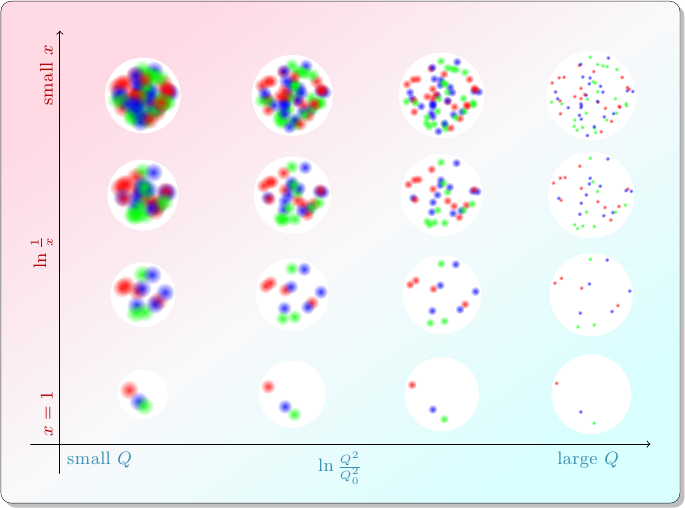
\includegraphics[width=0.9\textwidth]{xq2diagram-plain.png}
    \caption{\normalsize Diagram with the phase-space available through {\sffamily DIS}, in terms of $\ln{1/x}$ and $\ln{Q^2}$, taken from \cite{xq2diagrams}. A proton at low energies, consisting of three valence quarks, is shown in the left lower corner. As $Q$ increases, one may probe quarks with smaller transverse resolutions. As $x$ decreases, more gluons are produced until at very small-$x$ values a regime of gluon saturation is reached.}
\end{figure}

The study on how the parton distribution functions change when varying $Q^2$ and $x$ began with the {\sffamily DGLAP}\sidenote{Which describes to leading-logarithmic the evolution of {\sffamily PDFs} with increasing virtuality $Q^2$.}and {\sffamily BFKL}\sidenote{Describing how the gluon distribution functions change when going to smaller-$x$ values.}evolutions, constructed using perturbative {\sffamily QCD}. Nevertheless, the high-energy limit of {\sffamily QCD} may not be governed by the {\sffamily BFKL} equation since\sidenote{In the high-energy limit, this equation breaks the unitarity of the {\sffamily S} matrix and the Froissart bound on total cross section.}it does not incorporate the phenomena of {\sffamily\color{ming} gluon saturation}. As evidenced by the {\sffamily HERA} measurements \cite{Abramowicz:2015mha}, the gluon distribution function grows rapidly when going to smaller-$x$ values. Thus, the high-energy limit of {\sffamily QCD} should also be an evolution towards higher gluon densities.

Since the {\sffamily QCD} coupling constant in small at high energies, that is $\alpha \ll 1$, one would be tempted to assume that perturbation theory is applicable. Even though the system is weakly coupled, extremely high occupation numbers for the gluons may lead to an effective coupling of order unity at very small-$x$ values. On the other hand, high occupation numbers imply classical fields. This idea lead to the development \cite{mclerven1, mclerven2, mclerven3} of the {\sffamily MV} model, which along with the {\sffamily JIMWLK} evolution \cite{JalilianMarian:1997dw} are the fundamental components of {\sffamily CGC} \cite{iancunonlinear, Ferreiro:2001qy}, an effective theory for high-energy {\sffamily QCD}.

\begin{figure}[!hbt]
	\centering
    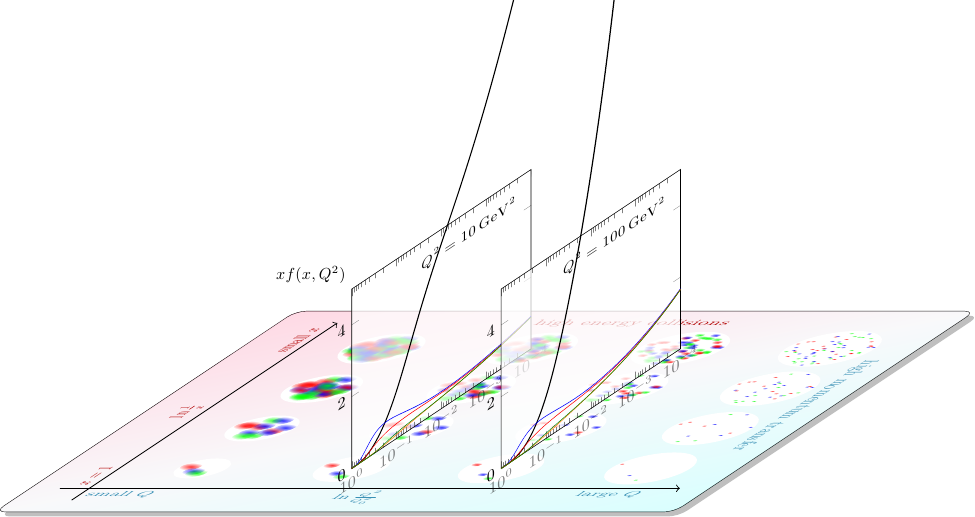
\includegraphics[width=\textwidth]{images/xq2diagram-pdfs.png}
    \caption{\normalsize Plots with parton distribution functions superimposed over the phase-space diagram of {\sffamily DIS}, for different values of $Q^2$, taken from \cite{xq2diagrams}. One may notice the dramatic growth of the gluon distribution function $xg(x,Q^2)$ when going to smaller-$x$ values.}
\end{figure}

